
\begin{figure}
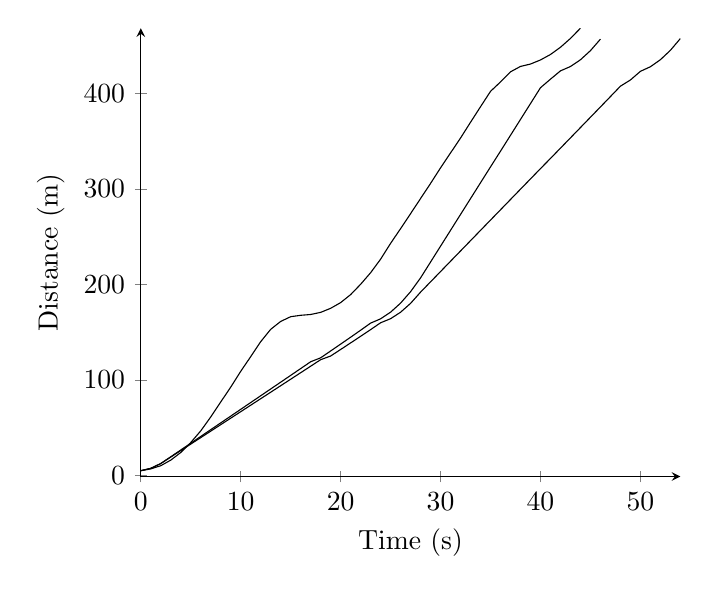
\begin{tikzpicture}
\begin{axis}[
legend style={
	anchor=west
},
axis x line=bottom,
axis y line=left,
ymin=-1,
point meta=explicit symbolic,
xlabel=Time (s),
ylabel=Distance (m)
]
\addplot[] coordinates {
(0, 5.1)
(1, 6.99374451642)
(2, 10.3551442385)
(3, 16.1747778488)
(4, 24.1367851267)
(5, 34.564339719)
(6, 46.761571307)
(7, 61.3486532592)
(8, 77.0289857131)
(9, 92.5456449056)
(10, 109.12199704)
(11, 124.490734208)
(12, 140.16456324)
(13, 153.078058104)
(14, 161.367620679)
(15, 166.33075482)
(16, 167.787662048)
(17, 168.631661777)
(18, 170.859754819)
(19, 175.101267165)
(20, 181.064755124)
(21, 189.436136419)
(22, 200.242185218)
(23, 212.361760411)
(24, 226.533242961)
(25, 243.108694658)
(26, 258.499694174)
(27, 274.204275768)
(28, 290.046313785)
(29, 305.861150598)
(30, 322.161342974)
(31, 337.782665322)
(32, 353.369975434)
(33, 369.875308047)
(34, 386.126481314)
(35, 402.231856898)
(36, 412.103913518)
(37, 422.662229041)
(38, 428.309779178)
(39, 430.802233438)
(40, 435.08859727)
(41, 440.810225012)
(42, 448.378402326)
(43, 457.625099521)
(44, 468.293666728)
};
\addplot[] coordinates {
(0, 5.1)
(1, 7.6)
(2, 12.6)
(3, 19.3820275515)
(4, 26.1647450381)
(5, 32.9482455497)
(6, 39.7326397365)
(7, 46.5180601621)
(8, 53.304667021)
(9, 60.0926557482)
(10, 66.8822672974)
(11, 73.6738022485)
(12, 80.4676405256)
(13, 87.2642695231)
(14, 94.0643251605)
(15, 100.868653413)
(16, 107.678405382)
(17, 114.495189543)
(18, 121.321326136)
(19, 125.16029471)
(20, 132.007601404)
(21, 138.882458552)
(22, 145.801675147)
(23, 152.80003356)
(24, 159.965864348)
(25, 164.238625799)
(26, 171.011387249)
(27, 180.2841487)
(28, 192.056910151)
(29, 202.831721207)
(30, 213.606560112)
(31, 224.381431022)
(32, 235.156338965)
(33, 245.931290082)
(34, 256.706291949)
(35, 267.481354025)
(36, 278.256488277)
(37, 289.031710069)
(38, 299.807039458)
(39, 310.582503138)
(40, 321.358137428)
(41, 331.99399305)
(42, 342.769989394)
(43, 353.549644554)
(44, 364.334507069)
(45, 375.12714369)
(46, 385.932142054)
(47, 396.758591423)
(48, 407.627421697)
(49, 414.140181672)
(50, 423.16408995)
(51, 428.000644781)
(52, 435.337199612)
(53, 445.173754442)
(54, 457.510309273)
};
\addplot[] coordinates {
(0, 5.1)
(1, 7.6)
(2, 12.6)
(3, 19.6902875193)
(4, 26.7813320534)
(5, 33.8732409692)
(6, 40.9661429758)
(7, 48.060193713)
(8, 55.1555831984)
(9, 62.2525458941)
(10, 69.35137454)
(11, 76.4524395132)
(12, 83.5562164787)
(13, 90.6633268106)
(14, 97.7745982736)
(15, 104.891158958)
(16, 112.014588016)
(17, 119.147168127)
(18, 123.292330849)
(19, 130.445503781)
(20, 137.625848173)
(21, 144.850117532)
(22, 152.153161507)
(23, 159.624067453)
(24, 164.094558872)
(25, 171.065050292)
(26, 180.535541711)
(27, 192.506033131)
(28, 206.97652455)
(29, 223.57652455)
(30, 240.17652455)
(31, 256.77652455)
(32, 273.37652455)
(33, 289.97652455)
(34, 306.57652455)
(35, 323.17652455)
(36, 339.63652455)
(37, 356.23652455)
(38, 372.83652455)
(39, 389.43652455)
(40, 406.03652455)
(41, 414.979661034)
(42, 423.664485432)
(43, 428.22034517)
(44, 435.276204909)
(45, 444.832064647)
(46, 456.887924386)
};

\end{axis}
\end{tikzpicture}
\label{tik:50:2_O, 2_O.-60, 4_S, 5_S, 5_S.-30, 6_V}
\caption{50 percent diving with GSC on route $2_O, 2_O.-60, 4_S, 5_S, 5_S.-30, 6_V$}
\end{figure}
